\documentclass[12pt,a4paper,spanish]{book}
\usepackage{fontspec}
\IfFileExists{../shared/fonts/Calibri/Calibri-Regular.ttf}{%
    \setmainfont[
        Path=../shared/fonts/Calibri/,
        Extension=.ttf,
        UprightFont=*-Regular,
        BoldFont=*-Bold,
        ItalicFont=*-Italic,
        BoldItalicFont=*-BoldItalic
    ]{Calibri}%
}{%
    \setmainfont{TeX Gyre Termes}%
}
\usepackage{../shared/estilo_unir-1}
\usepackage{braket}

\usepackage{tikz}
\usepackage{pgfplots}
\usepackage{float}
\pgfplotsset{compat=1.18}

\usepackage{setspace}
\onehalfspacing
\graphicspath{{fundamentos_de_mecanica_cuantica/images/}{images/}}

%---------------------------
%título del trabajo y autor
%---------------------------
\title{Actividad: Fundamentos de la mecánica cuántica}
\author{Francisco Javier Martínez Rodríguez, Ivan Dario Torres Garnica, Jeyson Antonio Flores Deras y José Juan Martínez Tapia}
\date{16 de febrero de 2026}
\profesor{Rodrigo Gil-Merino y Rubio}

%---------------------------
%marges
%---------------------------
%\usepackage[margin=1.9cm]{geometry}
%---------------------------
%---------------------------
%---------------------------
%---------------------------
\begin{document}
\renewcommand{\listfigurename}{Índice de figuras}
\renewcommand{\listtablename}{Índice de tablas}
\renewcommand{\contentsname}{Índice de contenidos}
\renewcommand{\figurename}{Figura}
\renewcommand{\tablename}{Tabla} 

\maketitle

\frontmatter
\tableofcontents
\listoffigures %atención, quitar si no hay figuras!!!
\listoftables %atención, quitar si no hay tablas!!!

\chapter{Resumen}

Este trabajo analizará la revolución conceptual que transformó la física entre finales del siglo XIX y principios del XX, cuando se empezaron a investigar y observar comportamientos que las reglas ``clásicas'' no podían explicar, como la famosa catástrofe ultravioleta, la cuantización de la energía~\cite{planckm1900_quantization_2}, el efecto fotoeléctrico~\cite{einsteina1905_photoelectric}, entre otros.

El objetivo es profundizar en el contexto histórico y el razonamiento detrás de cada uno de los hitos que dieron lugar al nacimiento de la ``mecánica cuántica antigua''. Al concluir este documento, el lector deberá comprender más a fondo y a detalle la historia detrás de cada descubrimiento.

El trabajo concluye en que esta transición hacia la mecánica de ondas no solamente resolvió las crisis a explorar, sino que estableció las bases indispensables de la computación cuántica, tema que abordaremos en futuras asignaturas (fuera del alcance de este documento).\\

{\bf Palabras clave:} Radiación de cuerpo negro, Cuantización, Ecuación de Schrödinger, Mecánica ondulatoria.\\

\chapter{Abstract}

This document will analyze the conceptual revolution that transformed physics between the late 19th and early 20th centuries, when scientists began observing and investigating unknown phenomena which the ``classical'' rules at that time could not explain, such as the ultraviolet catastrophe, the quantization of energy~\cite{planckm1900_quantization_2}, the photoelectric effect~\cite{einsteina1905_photoelectric}, amongst others.

The goal is to delve deeper into the historical context and the reasoning behind each one of these achievements that led to the origin of the ``old quantum theory''. Upon finishing this document, the reader should gain a deeper and more detailed understanding of the story behind each discovery.

This document concludes that the transition toward wave mechanics not only resolved the crises to be explored below, but also established the essential foundations of quantum computing, a topic we will address in future courses (out of this paper's scope).\\

{\bf Keywords:} Black-body radiation, Quantization, Schrödinger equation, Wave mechanics.\\

\mainmatter
\chapter{Introducción}

En la Introducción se debe resumir de forma esquemática pero suficientemente clara lo esencial de cada una de las partes del trabajo. La lectura de esta parte debe contextualizar perfectamente todo el trabajo y debe estar PLAGADA DE REFERENCIAS.\\

Las referencias NO están para rellenar. Son un TRIBUTO a las personas que hicieron en primer lugar una investigación o aportaron una idea, por tanto, se deben citar LOS TRABAJOS ORIGINALES DE LOS AUTORES, y no un libro de texto donde he visto que hablan de algo.\\

Es una parte muy importante de la memoria. Las ideas principales a transmitir son la identificación del problema a tratar, la justificación de su importancia, los objetivos generales a grandes rasgos y un adelanto de la contribución que esperas hacer.\\

A modo de guía, la Introducción debe contener estos tres apartados:
\begin{itemize}
\item Motivación / justificación del tema a tratar
\item Planteamiento del Trabajo
\item Estructura del Trabajo
\end{itemize}


ATENCIÓN:  Si queremos citar a alguien, por ejemplo porque vamos a hablar de Latex \citep{lamport1994} o porque, según las ideas de \cite{ackerman2017}, la liga de fútbol inglesa debe tener torneos de desempate, pues tenemos que hacerlo correctamente.



\chapter{Contexto y estado de la cuestión}\label{contexto}

En esta Sección~\ref{contexto} debemos demostrar que conocemos lo que se ha hecho en el ámbito que estamos desarrollando el Trabajo. En nuestro caso, que se ha buscado la bibliografía y referencias suficientes y que esas ideas se han volcado en el Trabajo en la línea de los objetivos que perseguimos o que queremos transmitir.


\chapter{Objetivos}

\section{Objetivo general}
Analizar la transición de la física cuántica partir de la radiación del cuerpo negro y su impacto en la comprensión de la luz, la estructura atómica y los modelos cuánticos.

\section{Objetivos específicos}

\begin{enumerate}
    \item Describir y analizar las principales leyes clásicas de la radiación térmica, incluyendo la ley de Stefan--Boltzmann (1879), la ley de desplazamiento de Wien (1893) y la formulación de Rayleigh--Jeans.
    
    \item Conceptualizar la crisis de la física clásica y naturaleza de la luz. Explicando el debate onda-corpúsculo y por qué las leyes de Newton/Maxwell fallaban a nivel atómico.
    
    \item Describir el efecto fotoeléctrico, experimento de la lámina de oro, átomo de Bohr, Sommerfeld y series de Balmer/Lyman y Mostrar la transición del modelo de "gelatina con pasas" al modelo planetario cuantizado.
    
    \item Analizar la ecuación de ondas de Schrödinger, orbitales de probabilidad y números cuánticos y Explicar cómo los electrones forman ondas estacionarias tridimensionales y sustituir las "órbitas" por "nubes de probabilidad".
\end{enumerate}

\chapter{Desarrollo del Trabajo}

\section{La Radiación del Cuerpo Negro: De lo Clásico a Planck.}

Planck desde joven se interesó en el estudio de la termodinámica, es decir el estudio de la relación entre el calor y
las diferentes formas de energía, este ámbito no solo tenía un enorme peso científico, sino que también concentraba una 
controversia fundamental sobre los principios que rigen la realidad física, Planck en búsqueda de la verdad, de lo absoluto, 
enseño al mundo las primeras pistas de la física cuántica.\par
\medskip


Planck en sus estudios universitarios tuvo el privilegio de conocer de primera mano los avances del electromagnetismo y 
termodinámica, ramas de la física esenciales para sus descubrimientos. Profundizando la comprensión del segundo principio, 
para el desarrollo de su investigación, donde dice que “En un sistema aislado la entropía siempre aumenta o, como mucho, permanece constante” 
términos que utilizo en sus trabajos sobre \textbf{la radiación del cuerpo negro} para explicar esto iniciaremos observando una chimenea, a medida que 
los troncos se calientan se pude observar un cambio de color a llamas más vivas, las zonas menos calientes no emiten luz visible aunque si nos calientan, 
la radiación la emite en radiación infrarroja que es invisible para el ojo humano, cuanto más caliente es el fuego más evoluciona su color de la 
luz emitida del rojo al azul, esto indica que cuanto más caliente esta un cuerpo, la luz que emite es más intensa y la longitud de onda es más pequeña. 
Entonces se generó un problema experimental concreto: determinar la distribución espectral de la radiación emitida por un cuerpo en equilibrio térmico, 
para mayor comprensión debemos plantearnos la siguiente pregunta ¿Qué es un cuerpo negro? Es un sistema ideal que debe cumplir dos características:

\begin{enumerate}
    \item Absorber toda la radiación incidente. (reflectiva nula)
    \item Emitir radiación con un espectro que depende únicamente de su temperatura.
\end{enumerate}

\begin{figure}[h]
    \centering
    \includegraphics[width=0.8\textwidth]{cavidad_aproximado_cuerpo_negro.png}
    \caption{Modelo de cavidad para aproximar a un cuerpo negro ideal. Fuente:\cite{planck1900}}
    \label{fig:espectro_cuerpo_negro}
\end{figure}

La radiación proveniente de una fuente externa entra por un orificio pequeño y sufre múltiples reflexiones en el interior de la cavidad. En cada reflexión, parte de la energía es absorbida por las paredes, de modo que la radiación incidente pierde progresivamente “memoria” de su dirección e intensidad inicial. Cuando el sistema alcanza equilibrio térmico, la cavidad reemite radiación electromagnética hacia el exterior, cuya distribución espectral depende principalmente de la temperatura de las paredes y se aproxima al espectro ideal de un cuerpo negro.  Fuente:\cite{planck1900}\par
\medskip


La magnitud fundamental que describe este fenómeno es la densidad \textbf{espectral de energía} por unidad de volumen: 

\begin{equation}
    u(v, T)
    \label{eq:densidad_espectral_energia}
\end{equation}

donde:

\begin{equation}
    \begin{aligned}
        v &= \text{frecuencia} \\
        T &= \text{temperatura absoluta}
    \end{aligned}
\end{equation}

Y la energía total viene dada por: 

\begin{equation}
    u(T)=\int_{0}^{\infty} u(\nu, T)\, d\nu
\end{equation}

El desafío consistía en encontrar la forma funcional correcta de \(u(\nu, T)\).

El problema del cuerpo negro era matemático, físico y conceptualmente complicado ya que se necesitaba del electromagnetismo (ecuaciones de maxwell), 
la mecánica estadística y el principio de equipartición de energía, este resultado dependía de una suposición implícita: La energía puede variar de 
forma continua, esto fue el origen de la crisis ya que la teoría clásica lograba explicar partes del comportamiento, pero no el conjunto completo, 
esto era una señal de que uno de los supuestos fundamentales de la física clásica estaba equivocado, esto representa uno de los momentos más importantes 
de la física porque mostro el límite de la mecánica clásica, revelo que el principio de equipartición no era universal e introdujo la idea revolucionaria 
de cuantización de la energía , esto consistió en abandonar la hipótesis de continuidad energética. 

\subsection{Ley de Stefan-Boltzmann}

La ley de Stefan-Boltzmann conecta de forma directa la temperatura de un cuerpo con la potencia total que emite en forma de radiación electromagnética, 
matemáticamente demuestra que la energía que emite un cuerpo está relacionada con su temperatura a las 4, cuanto más caliente este un objeto más energía 
radiara, esta demuestra que incluso pequeños aumentos en la temperatura conducen a grandes incrementos en la energía irradiada, esta ley surge antes de la 
existencia de la ,mecánica cuántica y antes de que se entendiera detalladamente la radiación del cuerpo negro, Josef Stefan la planteo basada en sus datos 
experimentales y poco después Ludwing Boltzmann lo sustento teóricamente basándose en la termodinámica y el electromagnetismo clásico, en términos físicos 
la ley dice que un objeto caliente emite radiación en todas las longitudes de onda y que la suma total de toda esa radiación depende fuertemente de la temperatura\cite{stefan1879}\par
\medskip

La ley establece que la \textbf{potencia total emitida por unidad de área} por un cuerpo negro es:

\begin{equation}
    M = \sigma T^4
\end{equation}

donde:
\begin{equation}
    \begin{aligned}
        M &= \text{potencia radiada por unidad de aréa (también llamada \textbf{exitancia radiante}) } [W\cdot m^{-2}] \\
        T &= \text{temperatura absoluta } [K] \\
        \sigma &= \text{\textbf{constante de Stefan-Boltzmann} } [W\cdot m^{-2}\cdot K^{-4}]
    \end{aligned}
\end{equation}

constante:
\begin{equation}
    \sigma = 5.670374419 \times 10^{-8} \, [W\cdot m^{-2}\cdot K^{-4}]
\end{equation}

Los materiales reales no son cuerpos negros perfectos. Se introduce la \textbf{emisividad} \(\varepsilon \) (entre 0 y 1)
para modelar cuánta radiación emite una superficie comparada con el cuerpo negro ideal:

\begin{equation}
    M = \varepsilon \sigma T^4
\end{equation}

Si el área es \(A\), la potencia total emitida es:

\begin{equation}
    \begin{aligned}
            P = A \cdot M \\
            P = A \cdot \varepsilon \sigma T^4
    \end{aligned}
\end{equation}

Esta ley tiene sus principales aplicaciones en la astrofísica (luminosidad estelar) la ingeniería térmica (perdidas radiactivas 
en hornos, turbinas, disipadores calientes), Clima y energía, su soporte practico como teórico es compatible con la teoría cuántica\cite{planck1900}.

\subsection{Ley de desplazamiento de Wien}

Cualquier cuerpo con temperatura mayor a cero emite radiación electromagnética esta emisión no ocurre en una sola magnitud de onda, sino cuya forma 
depende fuertemente de la temperatura, con la aparición del concepto de cuerpo negro Wien formulo una ley: a longitud de onda en la que el cuerpo negro 
emite con máxima intensidad se desplaza hacia longitudes de onda más cortas a medida que aumenta la temperatura, siguiendo una relación inversa\cite{wien1893}.\par
\medskip

La ley se expresa como:

\begin{equation}
    \lambda_{\text{max}} T = b
\end{equation}

donde:
\begin{equation}
    \begin{aligned}
        \lambda_{\text{max}} &= \text{longitud de onda en la que la emisión es máxima} \\
        T &= \text{temperatura absoluta del cuerpo} \\
        b &= \text{constante de desplazamiento de Wien}
    \end{aligned}
\end{equation}

constante:
\begin{equation}
    b = 2.897771955 \times 10^{-3} \, [m \cdot K]
\end{equation}

por tanto:
\begin{equation}
    \lambda_{\text{max}} = \frac{b}{T}
\end{equation}

En términos cualitativos: objetos fríos emiten principalmente en infrarrojo, mientras que objetos muy calientes emiten en visible o ultravioleta. La ley de Wien formaliza esta intuición y permite cuantificarla con una sola constante. 

% Figura
\begin{figure}[H]
    \centering
    {\bfseries Desplazamiento del máximo de emisión (Ley de desplazamiento de Wien)}\par
    \vspace{0.4em}
    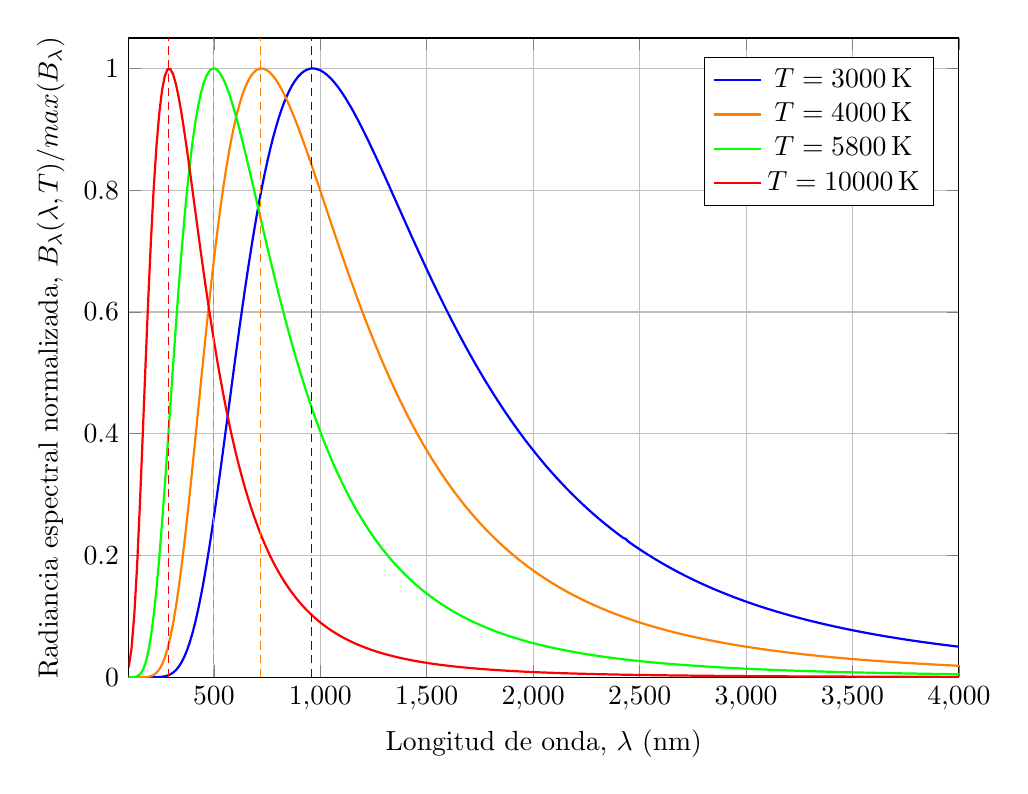
\begin{tikzpicture}
        \begin{axis}[
            width=\textwidth,
            height=0.8\textwidth,
            xlabel={Longitud de onda, \(\lambda\) (nm)},
            ylabel={Radiancia espectral normalizada, \(B_\lambda(\lambda,T)/{\text{max}}(B_\lambda)\)},
            xmin=100, xmax=4000,
            ymin=0, ymax=1.05,
            grid=both,
            legend pos=north east,
            domain=100:4000,
            samples=300
            ]   
            \pgfmathsetmacro{\cTwo}{1.438776877e-2}
            \pgfmathsetmacro{\bWien}{2.897771955e-3}
            \pgfplotsset{
                declare function={
                    planck(\x,\T)=1/((\x*1e-9)^5 * (exp(\cTwo/((\x*1e-9)*\T)) - 1));
                    lammax(\T)=\bWien/\T*1e9;
                    normplanck(\x,\T)=planck(\x,\T)/planck(lammax(\T),\T);
                }
            }
            \def\Ta{3000}
            \def\Tb{4000}
            \def\Tc{5800}
            \def\Td{10000}
            \addplot[thick, color=blue] {normplanck(x,\Ta)};
            \addlegendentry{\(T=\Ta\,\mathrm{K}\)}
            \addplot[thick, color=orange] {normplanck(x,\Tb)};
            \addlegendentry{\(T=\Tb\,\mathrm{K}\)}
            \addplot[thick, color=green] {normplanck(x,\Tc)};
            \addlegendentry{\(T=\Tc\,\mathrm{K}\)}
            \addplot[thick, color=red] {normplanck(x,\Td)};
            \addlegendentry{\(T=\Td\,\mathrm{K}\)}
            \addplot[densely dashed, color=blue] coordinates {(lammax(\Ta),0) (lammax(\Ta),1.05)};
            \addplot[densely dashed, color=orange] coordinates {(lammax(\Tb),0) (lammax(\Tb),1.05)};
            \addplot[densely dashed, color=green] coordinates {(lammax(\Tc),0) (lammax(\Tc),1.05)};
            \addplot[densely dashed, color=red] coordinates {(lammax(\Td),0) (lammax(\Td),1.05)};
        \end{axis}
    \end{tikzpicture}
    \caption{Espectros \(B_\lambda(\lambda,T)\) normalizados para distintas temperaturas, con líneas punteadas indicando \(\lambda_{\text{max}} = b/T \). Fuente: elaboración a partir de \cite{planck1901}.}
    \label{fig:wien_desplazamiento}
\end{figure}

En la figura (\ref{fig:wien_desplazamiento}), cada espectro se dividió por su valor máximo, de modo que todas las curvas alcanzan el valor 1 en su pico. Esto permite comparar exclusivamente la posición del máximo (y la forma relativa) sin que el aumento de magnitud con la temperatura oculte los detalles. Se aprecia que, al incrementar T, el pico migra hacia longitudes de onda más cortas: el espectro se “corre” hacia la izquierda. Este desplazamiento es la firma directa de la ley de Wien. Además, la anchura relativa del espectro cambia: a temperaturas más altas, la distribución mantiene un carácter amplio, pero con mayor peso relativo en el rango de \(\lambda\) cortas\cite{planck1901}. \par
\medskip

Esta ley tiene grandes aplicaciones, si se considera una estrella como un cuerpo negro, permite estimar una temperatura efectiva, este método ha sido fundamental en la clasificación estelar y en estimaciones iniciales de objetos irradiantes, También es utilizada en procesos industriales.\par
\medskip

\textbf{Ejercicio} (Ley de desplazamiento de Wien): temperatura de una estrella según su “color” (pico de emisión).\par
\medskip

Enunciado: una estrella presenta su maximo de emición en \(\lambda_{\text{max}} = 450 \, \text{nm}\) (zona azul del visible). Estima su temperatura superficial suponiendo que se comporta como un cuerpo negro.\par
\medskip

Datos: la constante de desplazamiento de Wien es \(b = 2.897771955 \times 10^{-3}\,\mathrm{m\,K}\).

\begin{equation}
    \lambda_{\max} T = b
    \label{eq:wien}
\end{equation}

Despejando la temperatura:

\begin{equation}
    T=\frac{b}{\lambda_{\max}}.
    \label{eq:wien_T}
\end{equation}

Para \(\lambda_{\max}=450\,\mathrm{nm}\), se convierte a metros:

\begin{equation}
    450\,\mathrm{nm} = 450\times10^{-9}\,\mathrm{m}=4.50\times10^{-7}\,\mathrm{m}.
    \label{eq:lambda_conversion}
\end{equation}

Sustituyendo en \eqref{eq:wien_T}:

\begin{equation}
    T=\frac{2.897771955\times10^{-3}\,\mathrm{m\,K}}{4.50\times10^{-7}\,\mathrm{m}}\approx 6.44\times10^{3}\,\mathrm{K}.
    \label{eq:wien_result}
\end{equation}

Por tanto, la temperatura correspondiente es \(T \approx 6.44\times10^{3}\,\mathrm{K}\) (aprox. \(6440\,\mathrm{K}\)).

\subsection{Ley de Rayleigh-Jeans y la catástrofe ultravioleta}

La ley de Rayleigh-Jeans constituye el intento clásico más influyente de derivar el espectro de radiación del cuerpo negro a partir de la mecánica estadística y la teoría electromagnética. Su importancia histórica radica en que reproduce con éxito el comportamiento experimental en el régimen de longitudes de onda grandes (bajas frecuencias), pero falla de manera dramática en el ultravioleta (altas frecuencias): predice una emisión que crece sin límite a medida que la longitud de onda disminuye. Esta divergencia recibe el nombre de catástrofe ultravioleta y fue una de las motivaciones directas para la introducción de la cuantización de la energía por Planck.\cite{rayleigh1900,jeans1905,planck1901}

Para calcular la densidad espectral de energía: forma en frecuencia y en longitud de onda, se identificará:

\begin{equation}
    u(\nu, T) = \text{como la densidad espectral de energía}
\end{equation}

\begin{equation}
    u(\nu, T)d\nu = \text{como la energía por volumen contenida entre } \nu \text{ y } \nu+d\nu.
\end{equation}

Planck en su artículo escribe que un puente técnico crucial es la relación de energía promedio U de un oscilador de frecuencia \(\nu\) y la densidad de energía radiactiva u a esa frecuencia:

\begin{equation}
    u(\nu, T) = \frac{8\pi\nu^2}{c^3} U(\nu, T)
\end{equation}

Planck la presenta como la ecuación (8) en su desarrollo, combinando relaciones de intensidad y densidad de energía. Esta relación es fundamental porque conecta la descripción microscópica (osciladores atómicos) con la macroscópica (radiación en el espacio), y es a través de esta conexión que Planck introduce la cuantización de la energía para resolver la catástrofe ultravioleta.\cite{planck1900}\par
\medskip

Ahora viene el paso clásico decisivo:\par
\medskip

En la física clásica, la energía media de un oscilador de frecuencia $\nu$ a temperatura $T$ viene dada por el teorema de equipartición:
\begin{equation}
    U(\nu,T)=\langle E\rangle = k_{B}T.
    \label{eq:cla_dec}
\end{equation}

Sustituyendo \eqref{eq:cla_dec} en la relación entre $u(\nu,T)$ y $U(\nu,T)$, se obtiene la ley de Rayleigh-Jeans:
\begin{equation}
    u(\nu,T)=\frac{8\pi\nu^{2}}{c^{3}}\,k_{B}T.
    \label{eq:rayleigh_jeans_u_nu}
\end{equation}

La “catástrofe ultravioleta” se hace visible al integrar la energía total predicha por Rayleigh-Jeans. La energía por unidad de volumen total sería:

\begin{equation}
    u_{\text{tot}}(T) = \int_{0}^{\infty} u(\nu,T)\,d\nu = \int_{0}^{\infty}\frac{8\pi\nu^{2}}{c^{3}}\,k_{B}T\,d\nu = \frac{8\pi k_{B}T}{c^{3}}\int_{0}^{\infty}\nu^{2}\,d\nu
\end{equation}

pero

\begin{equation}
    \int_{0}^{\infty}\nu^{2}\,d\nu = \lim_{N\to\infty}\int_{0}^{N}\nu^{2}\,d\nu = \lim_{N\to\infty}\frac{N^{3}}{3} = \infty
\end{equation}

En la física clásica teórica predice energía infinita cuando se permiten frecuencias arbitrariamente grandes, esto no concuerda con mediciones prácticas, el espectro real presenta un máximo y luego cae rápidamente por ello Planck en su artículo de 1901 enfatiza que las mediciones espectrales mostraban que leyes previas no eran universalmente validas, y que la teoría requería una corrección.\cite{planck1901}\par
\medskip

¿Que plantea Max Planck?\par 
\medskip

La ley de \cite{planck1900} es la relación matemática que describe, por primera vez de forma completa y en acuerdo con el experimento, cómo se distribuye la energía radiada por un cuerpo negro entre las distintas frecuencias, Explica que la formulación de Wien no es correcta para todo el espectro y Ryleigh-Jeans conduce a inconsistencias.

\section{El Fotón y la Estructura Nuclear: Einstein y Rutherford.}

\subsection{El Efecto Fotoeléctrico}
Según la teoría clásica, la luz es una perturbación periódica continua (u onda electromagnética) que se propaga en el espacio. Esta teoría predecía, por ejemplo, que en el efecto fotoeléctrico la energía de los electrones emitidos debería depender de la intensidad de la luz.
Sin embargo en el postulado del efecto fotoeléctrico ~\cite{einsteina1905_photoelectric} se demostró que la luz era de naturaleza corpuscular (formada por cuantos) así como la existencia de los fotones. A través de la experimentación se demostró que los electrones saltaban de forma instantánea y solo si la luz superaba una frecuencia umbral específica, independientemente de cuán intensa fuera la luz. Esta relación se expresa matemáticamente como:
\begin{equation}
    E_{\gamma} = h\nu = W_0 + E_{\text{cin}}
\end{equation}
Siendo que:
\begin{itemize}
\item $h\nu$ es la constante de Plank ($h$)~\cite{planckm1900_quantization_2} medida en Julios por segundo ($J \cdot s$) multiplicada por la frecuencia de la radiación ($\nu$) medida en segundos a la inversa ($s^{-1}$), generando que el resultado de la expresión sea en Julios ($J$).
\item $E_{\gamma}$ Es la energía del fotón incidente.
\item $W_0$ es la energía de extracción.
\item $E_{\text{cin}}$ es la energía cinética máxima de los electrones emitidos.
\end{itemize}
Esta formulación tiene la restricción de que $W_0$ debe ser mayor a $h\nu$ para que se produzca la emisión de electrones.

Teniendo en cuenta la estructura de la ecuación anterior, es posible calcular la frecuencia umbral necesaria para que se produzca el efecto fotoeléctrico, despejando la expresión para obtener $\nu$:
\begin{equation}
    \nu = \frac{W_0 + E_{\text{cin}}}{h}
\end{equation}
\section{El Átomo de Bohr-Sommerfeld y los Espectros Atómicos.}

Lorem ipsum dolor sit amet, consectetur adipiscing elit. Sed do eiusmod tempor incididunt ut labore et dolore magna aliqua. Ut enim ad minim veniam, quis nostrud exercitation ullamco laboris nisi ut aliquip ex ea commodo consequat. Duis aute irure dolor in reprehenderit in voluptate velit esse cillum dolore eu fugiat nulla pariatur.

\section{El Modelo de Schrödinger: Mecánica Ondulatoria.}

Esta sección explorará el contexto histórico y el razonamiento que dieron lugar a la famosa ecuación de ondas de Erwin Schrödinger~\cite{schrodinger1926}. Partiremos del acierto del modelo de Bohr respecto a que los niveles de energía del átomo podían cuantificarse (no obstante, aún sin fundamentos), hasta la construcción de la mecánica ondulatoria y orbital, y los trabajos subsecuentes.

\subsection{¿Qué pendientes dejaron los modelos de Bohr-Sommerfeld?}

Primero, recordemos que el modelo de \cite{rutherford1911} estableció que los electrones orbitan alrededor de un núcleo de carga positiva, y según la electrodinámica clásica, estos deberían de perder energía en forma de radiación contínua y caer al núcleo en cuestion de centésimas de nanosegundos; cosa que diverge de la realidad.

Bohr encontró una alternativa en 1913, postulando que los átomos tienen varios estados ``estacionarios'' en los que el electrón no produce radiación, y las órbitas solo pueden tener un momento angular múltiplo de \(\hbar\)~\cite{bohr1913}:

\begin{equation}
L = n \hbar
\label{eq:angular_momentum_rutherford}
\end{equation}

Con estos postulados obtuvo los niveles de energía del hidrógeno (\(E_n = -13.6/n^2\) eV) y explicó su espectro de emisión con notable precisión.

Posteriormente, \cite{sommerfeld1916} extendió el modelo permitiendo órbitas elípticas e introduciendo los números cuánticos azimutal \(\ell\) y magnético \(m\) mediante reglas de cuantización más generales:

\begin{equation}
E_n = -\frac{Z^2 e^4 m_e}{32\pi^2 \varepsilon_0^2 \hbar^2} \cdot \frac{1}{n^2}, \quad L = \ell\hbar, \quad L_z = m\hbar
\label{eq:sommerfeld}
\end{equation}

donde \(\ell\) describe la forma de la órbita (con valores \(0, 1, \ldots, n-1\)) y \(m\) su orientación espacial (con valores \(-\ell, \ldots, +\ell\)). Es importante recalcar que la energía \(E_n\) seguía dependiendo exclusivamente de \(n\), pues los números \(\ell\) y \(m\) no aparecían en la ecuación~\ref{eq:sommerfeld}. Esto implica que órbitas con formas y orientaciones distintas tienen la misma energía, algo que no coincidía con experimentos como el efecto Zeeman y la estructura fina, que mostraban desdoblamientos en las líneas espectrales que solo podían explicarse si la energía también dependía de \(\ell\) y \(m\).

Al igual que en el modelo de Bohr, los valores permitidos de \(\ell\) y \(m\) se imponen mediante reglas de cuantización sin una justificación teórica de fondo. Seguían siendo restricciones que funcionaban, pero que aún nadie podía derivar.

\subsubsection{Algunas limitaciones adicionales a lo anterior son:}

\begin{itemize}
    \item El modelo fallaba al describir átomos con más de un electrón.
    \item No se explicaba el mecanismo por el cual un electrón transiciona entre niveles de energía.
    \item El electrón se seguía tratando como una partícula puntual en una trayectoria definida.
\end{itemize}

Uno de los cuestionamientos más notables y conocidos fue el del propio Rutherford, quien en una carta dirigida a Bohr señaló: ``¿cómo decide un electrón a qué frecuencia va a vibrar cuando pasa de un estado estacionario a otro? Pareciera que se debe asumir que el electrón sabe de antemano dónde se va a detener''~\cite{rutherford1913carta}. \textbf{Hacía falta, por tanto, cambiar el panorama completo.}

\subsection{De Broglie y su razonamiento de la dualidad onda-partícula}

En 1905, Albert Einstein demostró que la luz—hasta entonces considerada exclusivamente como  una onda electromagnética—también se comportaba ocasionalmentecomo partícula (el fotón \(\gamma\) ), cuya energía viene dada por \(E = h\nu\)~\cite{einsteina1905_photoelectric}. En 1924, Louis de Broglie reflejó este razonamiento en su tesis doctoral: si las ondas pueden comportarse como partículas, ¿pueden las partículas comportarse como ondas?~\cite{debroglie1924}

\subsubsection{De Broglie propuso que toda partícula con momento \(p\) tiene asociada una longitud de onda \(\lambda\):}

\begin{equation}
\lambda = \frac{h}{p} = \frac{h}{m_e v}
\label{eq:debroglie}
\end{equation}

Esta hipótesis tuvo una consecuencia inmediata sobre el modelo de Bohr. Si el electrón es una onda, su órbita alrededor del núcleo debe contener un número entero de longitudes de onda para que la onda sea estacionaria—es decir, para que al completar una vuelta, la onda ``cierre'' sobre sí misma sin destruirse por interferencia destructiva. 

\begin{figure}[h]
    \centering
    \includegraphics[width=0.8\textwidth]{ondas_estacionarias_debroglie.png}
    \caption{Ondas estacionarias de de Broglie en órbitas de radio 
    creciente. Fuente: \cite{elert2024}.}
    \label{fig:debroglie_ondas}
\end{figure}

\noindent{Esta condición se expresa como:}

\begin{equation}
2\pi r = n\lambda = n\frac{h}{m_e v}
\label{eq:onda_estacionaria}
\end{equation}

\noindent{Al despejar, se obtiene directamente:}

\begin{equation}
m_e v r = n\hbar
\label{eq:bohr_desde_debroglie}
\end{equation}

que es precisamente la condición de cuantización del momento angular que Bohr había postulado como restricción once años antes. Lo que en el modelo de Bohr era un hecho sin precedentes, en el razonamiento de de Broglie se convertía en una consecuencia natural de la naturaleza ondulatoria del electrón.

Sin embargo, mientras la onda del electrón se seguía tratando como unidimensional, envuelta alrededor de una trayectoria circular, un electrón real existe en tres dimensiones, y su comportamiento ondulatorio debería describirse mediante una ecuación de ondas tridimensional—análoga a las ecuaciones de Maxwell para la luz. Como señala el material del curso, ``Schrödinger aprovecha la idea de De Broglie de asociar una onda a cada partícula, y desarrolla una ecuación de ondas que deben cumplir todas las partículas que pudiesen representarse mediante una función de onda \(\Psi\)''~\cite{tema2}.

\subsection{La ecuación de onda de Schrödinger}

Ante las limitaciones de la teoría cuántica antigua, surgieron dos enfoques para construir una mecánica cuántica completa. En 1925, Werner Heisenberg propuso trabajar directamente con matrices de magnitudes observables, dando lugar a la mecánica matricial~\cite{heisenberg1925}. De forma independiente, Erwin Schrödinger partió de la hipótesis de de Broglie y desarrolló una ecuación de ondas que toda partícula debía satisfacer~\cite{schrodinger1926}. Aunque los dos caminos parecían muy distintos, el propio Schrödinger demostró que eran matemáticamente equivalentes~\cite{tema2}. Como ejemplo, el momento angular \(L_z\) en ambas representaciones se expresa como:

\begin{equation}
\text{Heisenberg: } L_z = Q_x P_y - Q_y P_x
\label{eq:heisenberg_lz}
\end{equation}

\begin{equation}
\text{Schrödinger: } L_z = -i\hbar\left(x\frac{\partial}{\partial y} - y\frac{\partial}{\partial x}\right)
\label{eq:schrodinger_lz}
\end{equation}

En ambos casos, la estructura es la misma: posición en \(x\) por momento en \(y\), menos posición en \(y\) por momento en \(x\). Heisenberg representa la posición (\(Q\)) y el momento (\(P\)) como matrices, mientras que Schrödinger representa la posición como la coordenada \(x\) y el momento como el operador diferencial \(-i\hbar\,\partial/\partial x\).

\noindent Centrando la atención en el enfoque ondulatorio, la ecuación de Schrödinger en su forma completa es:

\begin{equation}
i\hbar\frac{\partial}{\partial t}\Psi(\mathbf{r},t) = -\frac{\hbar^2}{2m}\nabla^2\Psi(\mathbf{r},t) + U(\mathbf{r})\Psi(\mathbf{r},t)
\label{eq:schrodinger_td}
\end{equation}

donde \(\Psi(\mathbf{r},t)\) es la función de onda de la partícula, \(m\) su masa, \(U(\mathbf{r})\) el potencial al que está sometida, y \(\nabla^2\) es el operador laplaciano. El lado izquierdo describe cómo evoluciona \(\Psi\) en el tiempo. En el lado derecho, el primer término representa la energía cinética y el segundo la energía potencial.

Cuando el potencial no depende del tiempo—como ocurre con la interacción coulombiana entre el electrón y el núcleo—la función de onda puede separarse en dos partes independientes:

\begin{equation}
\Psi(\mathbf{r},t) = \psi(\mathbf{r})\,\phi(t)
\label{eq:separacion}
\end{equation}

La parte temporal tiene una solución directa, \(\phi(t) = e^{-iEt/\hbar}\), que al calcular la densidad de probabilidad \(|\Psi|^2 = |\psi|^2 \cdot |\phi|^2\) desaparece, ya que \(|e^{-iEt/\hbar}|^2 = 1\). Esto significa que la distribución de probabilidad no cambia con el tiempo, lo cual justifica el nombre de ``estados estacionarios'' que Bohr había introducido en 1913~\cite{bohr1913}: ahora, en vez de ser un postulado, es una consecuencia matemática de la ecuación.

\noindent La parte espacial satisface la ecuación de Schrödinger independiente del tiempo:

\begin{equation}
E\psi(\mathbf{r}) = -\frac{\hbar^2}{2m}\nabla^2\psi(\mathbf{r}) + U(\mathbf{r})\psi(\mathbf{r})
\label{eq:schrodinger_ti}
\end{equation}

Esta es la ecuación que se resuelve para obtener los niveles de energía \(E\) y las funciones de onda \(\psi(\mathbf{r})\) permitidas. A diferencia de los modelos de Bohr y Sommerfeld, la cuantización no se impone: emerge naturalmente de las condiciones de contorno que debe satisfacer \(\psi\) (ser finita, continua y normalizable). En el modelo de Schrödinger, las órbitas del electrón son sustituidas por \textit{orbitales} espaciales que representan la probabilidad de encontrar al electrón en un punto del espacio~\cite{tema2}.


\subsection{Solución para el hidrógeno: números cuánticos, orbitales y nubes de probabilidad}

Para aplicar la fórmula anterior al átomo del hidrógeno, se toma en cuenta que la energía potencial \(U(r)\)  es la de Coulomb: \(-e^2/(4\pi\varepsilon_0 r)\). Ya que esto depende únicamente de la distancia \(r\) al núcleo, podemos restructurar en coordenadas esféricas \((r, \theta, \phi)\), donde la función de onda puede representarse en dos partes:

\begin{equation}
\psi(r,\theta,\phi) = R_{n,\ell}(r) \cdot Y_\ell^{m}(\theta,\phi)
\label{eq:separacion_esferica}
\end{equation}

\(R(r)\), describe cómo varía la probabilidad con la distancia al núcleo. La otra, \(Y(\theta,\phi)\), describe cómo varía con la dirección.

Como ecuación matemática, la ecuación de Schrödinger admite soluciones para cualquier valor de energía. Sin embargo, la mayoría de estas soluciones no describen un electrón real: algunas divergen al infinito, otras presentan discontinuidades, y otras dan probabilidades totales distintas de 1. Al descartar estas soluciones no físicas y quedarnos únicamente con aquellas que son finitas, continuas y normalizables, solo sobreviven soluciones para ciertos valores discretos de energía y momento angular. Estos valores quedan etiquetados por tres números cuánticos:

\begin{itemize}
\item \(n = 1, 2, 3, \ldots\) (principal): determina la energía del electrón, \(E_n = -13.6/n^2\) eV. Surge de la parte radial \(R(r)\) de la función de onda.
\item \(\ell = 0, 1, \ldots, n-1\) (azimutal): determina el momento angular orbital \(L = \sqrt{\ell(\ell+1)}\,\hbar\) y define las subcapas \(s, p, d, f\). Surge de la parte angular \(Y(\theta, \phi)\).
\item \(m_\ell = -\ell, \ldots, +\ell\) (magnético): determina la orientación del momento angular en el espacio, \(L_z = m_\ell\hbar\). Explica el efecto Zeeman. También surge de la parte angular.
\end{itemize}

Es decir, cada número cuántico aparece porque la función de onda, al tener que cumplir condiciones físicas en una geometría esférica, solo ``encaja'' para ciertos valores.

\begin{figure}[h]
    \centering
    \includegraphics[width=0.7\textwidth]{orbitales_schrodinger_born.png}
    \caption{Orbitales atómicos de Schrödinger-Born, etiquetados por \((n, \ell, m)\). Fuente: \cite{malgieri2022}.}
    \label{fig:orbitales}
\end{figure}

La interpretación física de \(\psi\) fue proporcionada por \cite{born1926}: \(|\psi(\mathbf{r})|^2\) representa la densidad de probabilidad de encontrar al electrón en la posición \(\mathbf{r}\). Las ``órbitas'' definidas del modelo de Bohr se transforman en nubes de probabilidad tridimensionales—los orbitales. Los orbitales \(s\) (\(\ell = 0\)) son esféricos, los \(p\) (\(\ell = 1\)) tienen forma bilobular, y los \(d\) (\(\ell = 2\)) presentan formas cuadrilobulares.

Un cuarto número cuántico, el espín (\(m_s = \pm 1/2\)), fue introducido por \cite{pauli1925} para explicar la estructura fina de los espectros. Pauli además enunció su principio de exclusión: dos electrones en un átomo no pueden compartir los mismos cuatro números cuánticos. Esto limita cada orbital a dos electrones con espines opuestos y determina la capacidad de cada capa electrónica: \(2n^2\) electrones. El llenado progresivo de orbitales según este principio reproduce la estructura de la tabla periódica: los bloques \(s\), \(p\), \(d\) y \(f\) corresponden directamente a los valores de \(\ell\).

\subsection{¿Qué pendientes dejó el trabajo de Schrödinger?}

A pesar de representar un salto importante respecto a la teoría cuántica antigua, el modelo de Schrödinger presenta limitaciones que el propio material del curso identifica~\cite{tema2}:

\begin{itemize}
\item No incorpora el espín electrónico de forma natural. El espín fue introducido por Pauli como un postulado adicional~\cite{pauli1925}, pero no emerge de la ecuación de Schrödinger.
\item No contempla efectos relativistas. Para electrones en átomos pesados, donde las velocidades son una fracción significativa de la velocidad de la luz, la ecuación pierde precisión ya que se da por hecho que la masa del electrón es constante.
\item No explica el mecanismo por el cual un electrón salta de un nivel energético a otro.
\end{itemize}

Las dos primeras limitaciones fueron resueltas por Paul Dirac en 1928, quien formuló una ecuación que unifica la mecánica cuántica con la relatividad especial. De esta ecuación, el espín y la existencia de la antimateria emergen como consecuencias naturales de la teoría, de la misma forma en que los números cuánticos \(n\), \(\ell\) y \(m\) emergen de la ecuación de Schrödinger.

No obstante, la mecánica ondulatoria de Schrödinger estableció un cambio de paradigma que permanece vigente: los electrones no son partículas puntuales en órbitas definidas, sino distribuciones de probabilidad descritas por funciones de onda. Los números cuánticos no son postulados arbitrarios, sino consecuencias matemáticas de las condiciones de contorno. Y la estructura de la materia—desde el átomo de hidrógeno hasta la tabla periódica—emerge de una sola ecuación diferencial y un principio de exclusión. Estas ideas constituyen los cimientos sobre los que se construye la computación cuántica, tema que se abordará en asignaturas posteriores de este máster.

\chapter{Conclusiones}

Las Conclusiones es otra parte muy IMPORTANTE de la memoria. Deben ser muy clara. Si es posible se pueden itemizar o, mejor, poner un párrafo por idea con un pequeño título ilustrativo.

\addcontentsline{toc}{chapter}{Bibliografía}
\begin{thebibliography}{a}

%%\bibitem{etiqueta} \textsc{Autores},\textit{nombre referencia.}Información addicional

\bibitem[(Bohr, 1913)]{bohr1913} Bohr, N. (1913). On the constitution of atoms and molecules. \emph{Philosophical Magazine}, \emph{26}(151).

\bibitem[Born(1926)]{born1926} Born, M. (1926). Zur Quantenmechanik der Stoßvorgänge [Sobre la mecánica cuántica de los procesos de colisión]. \emph{Zeitschrift für Physik}, \emph{37}(12).

\bibitem[(de Broglie, 1924)]{debroglie1924} de Broglie, L. (1924). Recherches sur la théorie des quanta [Investigaciones sobre la teoría de los cuantos] (Tesis doctoral). Université de Paris.

\bibitem[(Einstein, 1905)]{einsteina1905_photoelectric} Einstein, A. (1905). Über einen die Erzeugung und Verwandlung des Lichtes betreffenden heuristischen Gesichtspunkt [Sobre un punto de vista heurístico relativo a la producción y transformación de la luz]. \emph{Annalen der Physik}.

\bibitem[(Elert, 2024)]{elert2024} Elert, G. (2024). Atomic Models. \emph{The Physics Hypertextbook}. https://physics.info/atomic-models/

\bibitem[(Gil-Merino, 2026)]{tema2} Gil-Merino, R. (2026). Tema 2: Teoría de la Radiación. \emph{Fundamentos de la Mecánica Cuántica}, Universidad Internacional de La Rioja (UNIR).

\bibitem[(Heisenberg, 1925)]{heisenberg1925} Heisenberg, W. (1925). Über quantentheoretische Umdeutung kinematischer und mechanischer Beziehungen [Sobre la reinterpretación cuántico-teórica de relaciones cinemáticas y mecánicas]. \emph{Zeitschrift für Physik}, \emph{33}(1).

\bibitem[(Malgieri, 2022)]{malgieri2022} Malgieri, M. (2022). What Schrödinger's cat tells us about the relationship between physics and philosophy. \emph{ResearchGate}. https://www.researchgate.net/publication/381897611

\bibitem[Pauli(1925)]{pauli1925} Pauli, W. (1925). Über den Zusammenhang des Abschlusses der Elektronengruppen im Atom mit der Komplexstruktur der Spektren [Sobre la conexión entre la completitud de los grupos de electrones en el átomo con la estructura compleja de los espectros]. \emph{Zeitschrift für Physik}, \emph{31}(1).

\bibitem[(Planck, 1900)]{planckm1900_quantization_2} Planck, M. (1900). Zur Theorie des Gesetzes der Energieverteilung im Normalspectrum [Sobre la teoría de la ley de distribución de energía en el espectro normal]. \emph{Verhandlungen der Deutschen Physikalischen Gesellschaft}.

\bibitem[Rutherford(1911)]{rutherford1911} Rutherford, E. (1911). The scattering of \(\alpha\) and \(\beta\) particles by matter and the structure of the atom. \emph{Philosophical Magazine}, \emph{21}(125).

\bibitem[(Rutherford, 1913)]{rutherford1913carta} Rutherford, E. (1913). Carta a N. Bohr. Reproducida en \emph{Physics of the Atom}. Publicada en \emph{Proceedings of the Physical Society}, \emph{78}(6).

\bibitem[(Schrödinger, 1926)]{schrodinger1926} Schrödinger, E. (1926). Quantisierung als Eigenwertproblem [Cuantización como problema de valores propios]. \emph{Annalen der Physik}.

\bibitem[Sommerfeld(1916)]{sommerfeld1916} Sommerfeld, A. (1916). Zur Quantentheorie der Spektrallinien [Sobre la teoría cuántica de las líneas espectrales]. \emph{Annalen der Physik}, \emph{356}(17).

\bibitem[(Stefan, 1879)]{stefan1879} Stefan, J. (1879). Über die Beziehung zwischen der Wärmestrahlung und der Temperatur.

\bibitem[(Wien, 1893)]{wien1893} Wien, W. (1893). Die obere Grenze der Wellenlängen, welche in der Wärmestrahlung fester Körper vorkommen können; Folgerungen aus dem zweiten Hauptsatz der Wärmetheorie.

\bibitem[(Planck, 1900)]{planck1900} Planck, M. (1900). Zur Theorie des Gesetzes der Energieverteilung im Normalspektrum.

\bibitem[(Planck, 1901)]{planck1901} Planck, M. (1901). On the Law of Distribution of Energy in the Normal Spectrum [Traducción fiel de la publicación alemana]. \emph{Annalen der Physik}.

\bibitem[(Rayleigh, 1900)]{rayleigh1900} Rayleigh, Lord (1900). On the light from the sky, its polarization and colour. \emph{Philosophical Magazine}.

\bibitem[(Jeans, 1905)]{jeans1905} Jeans, J. H. (1905). On the partition of energy between matter and ether. \emph{Philosophical Magazine}.

\end{thebibliography}
%\bibliographystyle{plain} 
%\bibliography{bibliografia}


\appendix
\chapter{Apéndices}

El modelo de \cite{rutherford1911} estableció que los electrones orbitan alrededor de un núcleo de carga positiva. Sin embargo, según las leyes de la electrodinámica clásica, un electrón en movimiento orbital debería emitir radiación de forma continua, perder energía, y caer en espiral hacia el núcleo. \textbf{Esto, evidentemente, no ocurre.}

\begin{figure}[h]
    \centering
    \includegraphics[width=0.8\textwidth, height=0.2\textwidth]{espectroscopia_emision_h.jpg}
    \caption{Espectro de emisión del hidrógeno.}
    \label{fig:espectro_h}
\end{figure}

Asimismo, Bohr, al observar que las frecuencias del espectro de emisión del hidrógeno (Figura~\ref{fig:espectro_h}) no se podían explicar si se consideraba a la energía del electrón (y por ende, radiación) como un rango continuo, determinó que las líneas espectrales correspondían a la radiación emitida cuando un electrón transicionaba entre dos estados de energía discretos indicados por el número cuántico \(n\)~\cite{bohr1913}. La energía de estos estados viene dada:

\begin{equation}
E_n = -\frac{E_0}{n^2}, \quad \textit{donde } E_0 = \frac{e^4 m_e}{8\varepsilon_0^2 h^2} = 13.6 \text{ eV}
\label{eq:energia_bohr}
\end{equation}

\(E_0\) es la energía del estado fundamental del átomo de hidrógeno, que resulta de combinar la energía cinética y potencial coulombiana del electrón con la condición de cuantización del 
momento angular (el momento angular se expresa por \(L = n\hbar\); es decir, por cuantos de \(\hbar\)). La energía del fotón emitido durante la transición entre dos estados estacionarios es:

\begin{equation}
E_{\textit{fotón}} = E_i - E_f = h\nu
\end{equation}

Donde:
\begin{itemize}
\item \(E_i\) : energía del estado inicial del electrón, donde \(E_i > E_f\)
\item \(E_f\) : energía del estado final del electrón.
\item \(h = 6.626 \times 10^{-34}\) J \(\cdot\) s : constante de Planck.
\item \(\nu\) : frecuencia del fotón emitido.
\end{itemize}

\end{document}